\section{The Elder Problem}
%\large{\bf Benchmark to verify density-dependent flow}\\
%by Chan-Hee Park.\\ 
%\normalsize
%\subsection{Definition}
%\begin{description}
%  \item[Purpose:] 
\subsection{Definition}
The Elder problem is a benchmark to verify density-dependent flow such as free convection, seawater intrusion, and possibly enhanced gas recovery with CO2.
%\item[Model description:] 
\paragraph*{Model description.}
The Elder Problem is a good example of free convection phenomena, where the fluid flow is driven purely by the density differences of the fluids. Figure \ref{ElderProblemBC} illustrates the boundary conditions of the Elder problem. Table \ref{TableElder} presents the specific parameters for the Elder problem used in this application.
%\end{description}
\begin{figure}[h]
\centering
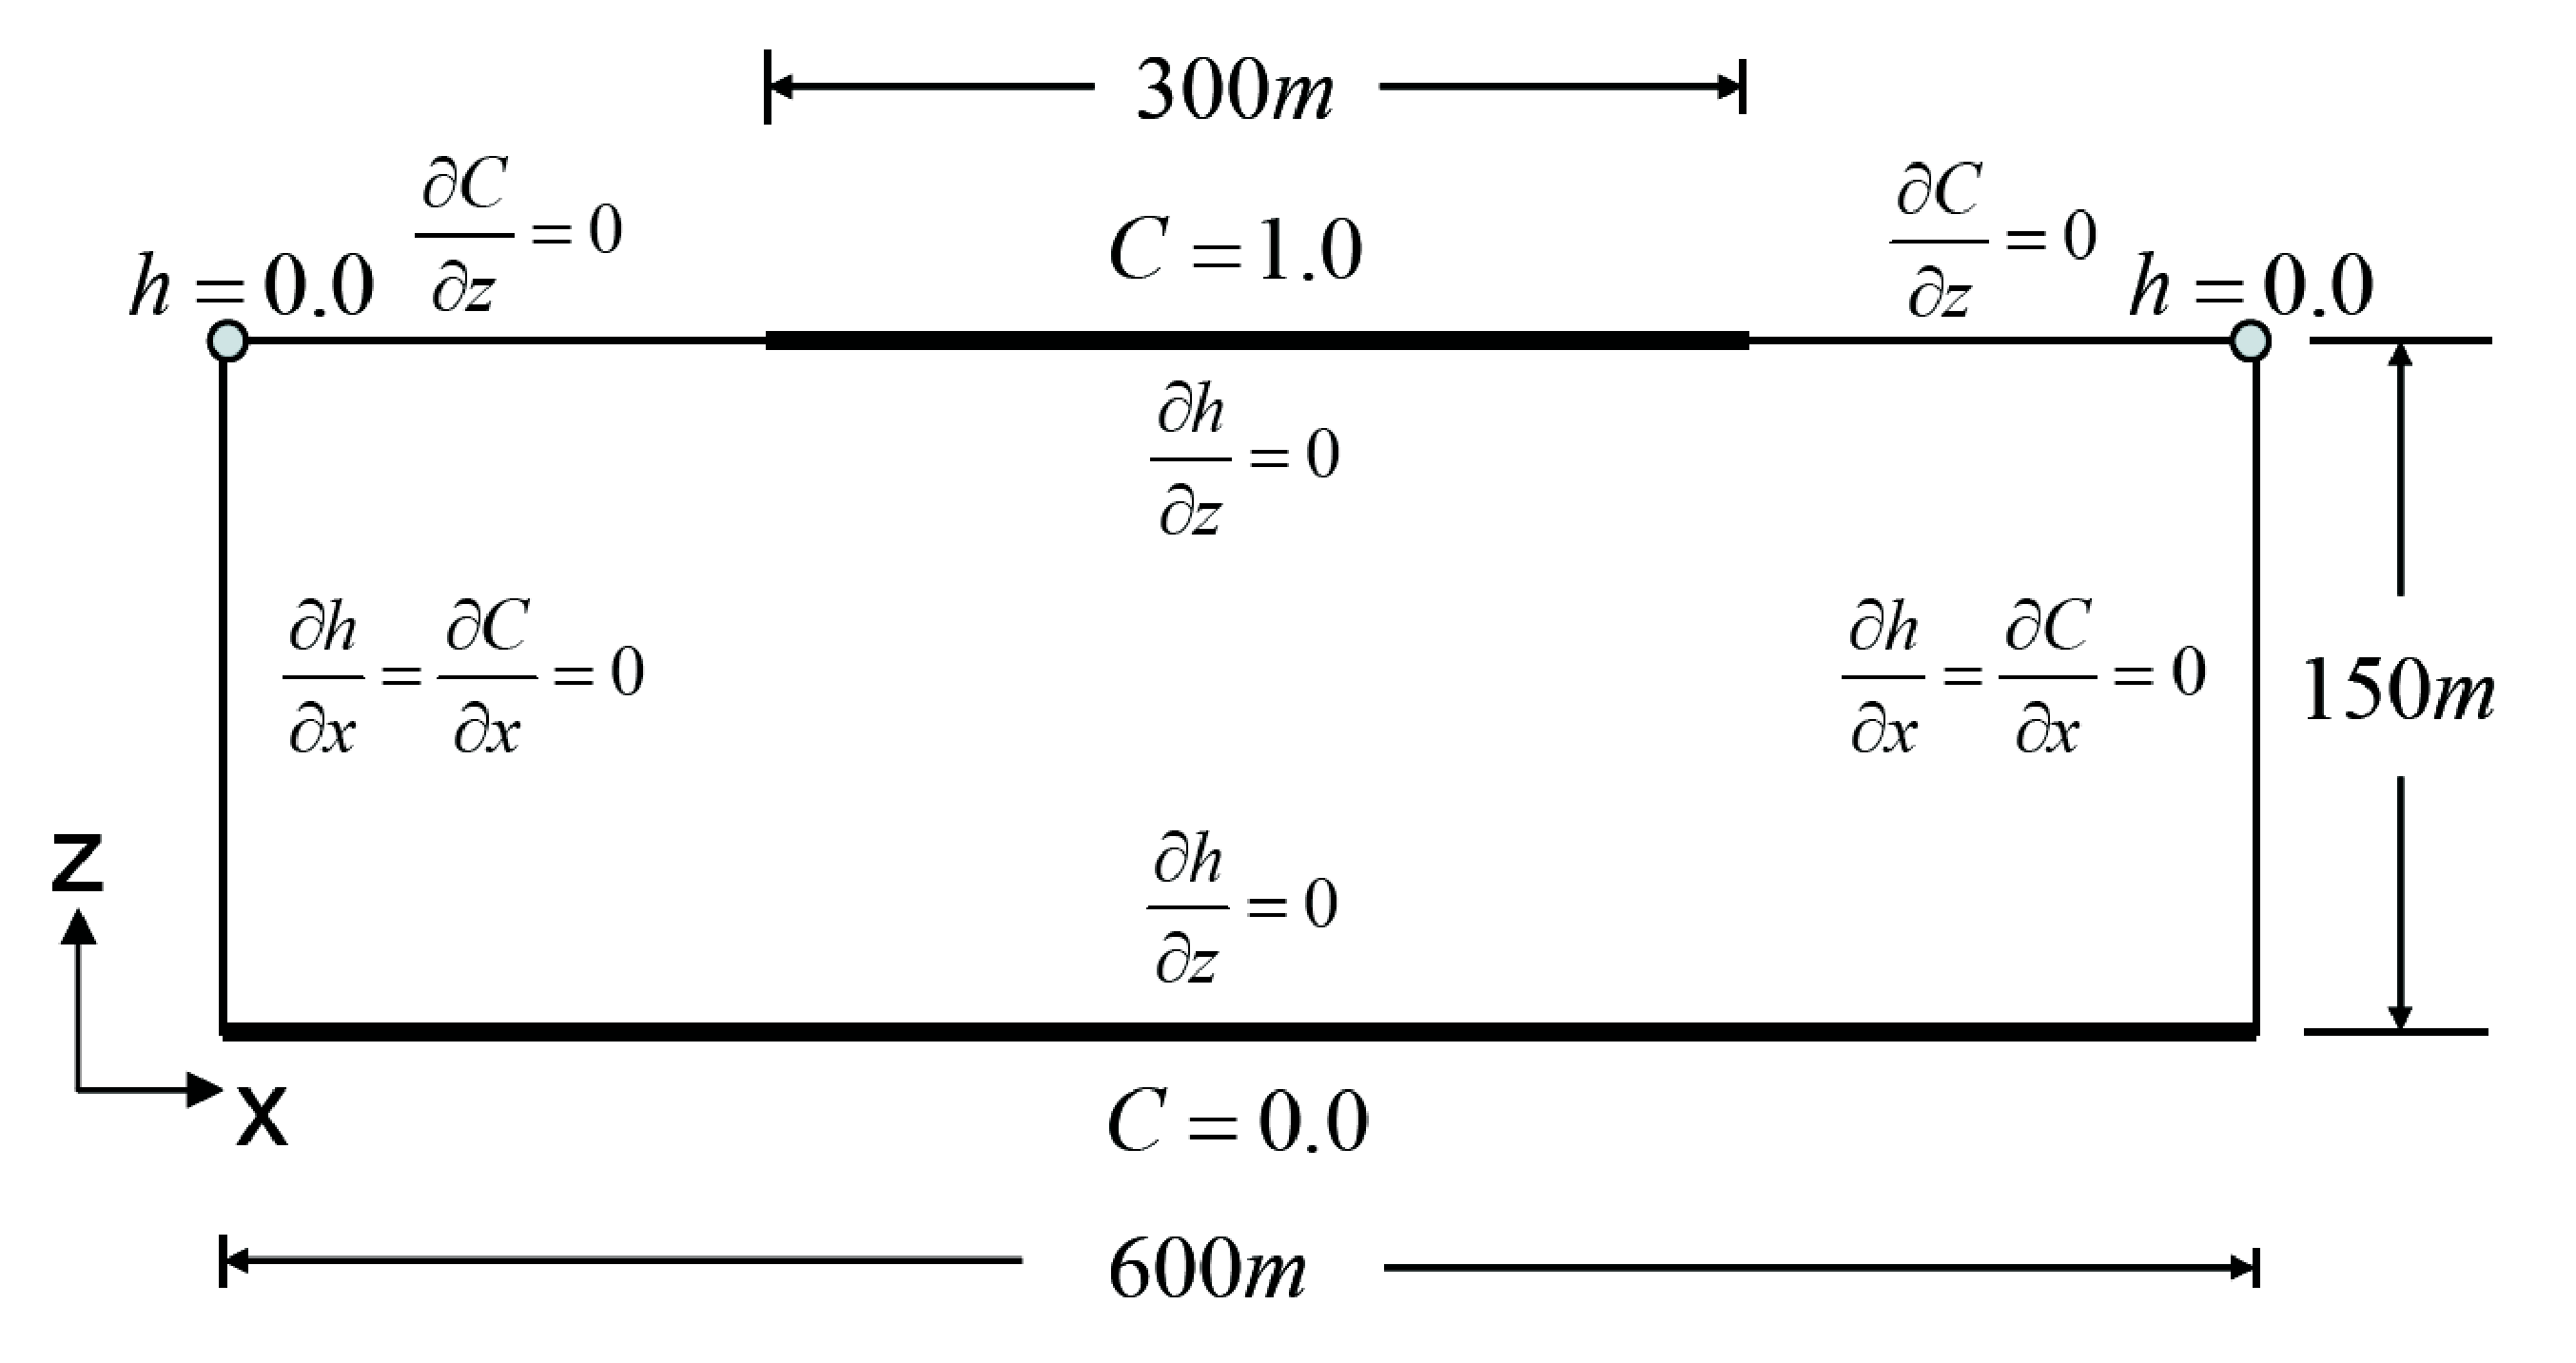
\includegraphics[scale=0.25]{PART_III/DDF/figures/elder_bc.eps}
\caption{Boundary conditions of the Elder problem}
\label{ElderProblemBC}
\end{figure}

\begin{table}[H]
\begin{center}
\begin{tabular}{llll}
\hline \hline
Symbol & Quantity   &  Value  & Unit\\
\hline \hline
 $D _m$ & Molecular diffusion coefficient & 3.565e-6  &  $m^2 s^{ - 1}$ \\
 $k$ & Permeability & 4.845e-13  &  $m^2$ \\
 $\mu$ & Dynamic viscosity & 10e-6  &  $kg m^{ - 1} s^{ - 1}$ \\
 $g$ & Gravitational coefficient & 9.81  &  $m s^{ - 2}$ \\
 $\alpha _L , \alpha _T$ & Longitudinal and transverse dispersivity & 0, 0  &  $m$ \\
 $\phi$ & porosity & 0.1  &  $-$ \\
 $\rho _0 , \rho _s$ & Density of water and saltwater & (1,1.2)e3  &  $kg m^{ - 3}$ \\
\hline \hline
\end{tabular}
\end{center}
\caption{Parameters for the Elder problem} \label{TableElder}
\end{table}


\subsection{Results}

The mesh was created with hexahedral elements for further expansion to 3D applications. The grid density level is defined as the $l$th level that consists of $2^{2l+1}$ identical square elements. Based on the definition of the grid density, the number of the hexahedral elements is 8192. The isochlor is defined as a ratio of a density difference to the maximum density difference. Figure \ref{ElderResult} shows the numerical results obtained from \textsc{OpenGeoSys} as the solution of the Elder problem.
%-------------------------------------------------

\begin{figure}[h]
\centering
\includegraphics[scale=0.22]{PART_III/DDF/figures/ElderResult.eps}
\caption{Isochlors of the Elder problem for 1, 2, 10, and 20 year at
regular grid of level 6} \label{ElderResult}
\end{figure}